\documentclass[10pt]{article}
\usepackage[margin=1in]{geometry}
\usepackage[T1]{fontenc}
\usepackage[utf8]{inputenc}
\usepackage{lmodern}
\usepackage{microtype}
\usepackage{booktabs}
\usepackage{graphicx}
\usepackage{float}
\usepackage{hyperref}
\usepackage{enumitem}
\usepackage{array}

\title{\textbf{Mini-Project\\Consumer Complaint Classification under Small-Data Constraints}\\
Natural Language Processing (NLP) in Python}
\author{Students: Khayrislamov Timur, Petrenko Maksim \\ Instructor: Assoc. Prof. Soroosh Shalileh}
\date{}

\begin{document}
\maketitle

\begin{abstract}
This mini-project studies text classification on consumer finance complaints under small-data conditions. We compare a classical sparse baseline (\textit{TF--IDF + Logistic Regression}) against two embedding-based approaches: \textit{Local Word2Vec + MLP} and \textit{Pretrained GloVe + MLP}. The main task is to predict the complaint product category from the complaint narrative. To make the evaluation more reliable, we test multiple balanced subset sizes and average the results over three random seeds. Across all settings, TF--IDF + Logistic Regression is the strongest model. Local Word2Vec improves substantially as more domain data becomes available and consistently outperforms pretrained GloVe. The results suggest that this classification problem is highly lexicalized and that domain-specific representations are more useful than general-purpose pretrained embeddings, although neither embedding-based model surpasses the classical baseline.
\end{abstract}

\section{Introduction}
A common assumption in modern NLP is that dense word embeddings should outperform traditional bag-of-words features, especially when the amount of labeled data is limited. However, this assumption does not always hold in applied classification tasks where the label can often be inferred from highly discriminative lexical patterns. Consumer complaint narratives are a good example of this setting: the text is noisy and varied, but it often contains strong domain-specific cues such as product names, recurring legal or financial terms, and repeated complaint formulations.

The goal of this project is to compare classical and embedding-based text representations on a realistic complaint classification problem. More specifically, we ask two questions: (1) how performance changes as the number of labeled examples per class increases, and (2) whether pretrained embeddings are more effective than locally trained embeddings in the low-data regime.

\section{Dataset and Task}
The experiments use the \texttt{Consumer Complaint} dataset. From the raw file, we selected the top five product categories with sufficient data and retained only rows with non-empty \texttt{consumer\_complaint\_narrative}. We also kept the \texttt{issue} field for filtering and possible qualitative analysis, but the main prediction target in this project is \texttt{product}.

To make the setup balanced and suitable for controlled experiments, we constructed a balanced dataset with up to 2000 examples per class in the final study. After filtering, text cleaning, and class balancing, the task becomes a 5-class text classification problem. The input is the complaint narrative, and the output is the product category.

The text preprocessing pipeline includes lowercasing, removing placeholder tokens such as \texttt{XXXX}, deleting URLs and emails, removing digits, removing non-alphabetic characters, collapsing whitespace, and discarding very short cleaned texts.

\section{Models}
We compare three models.

\paragraph{TF--IDF + Logistic Regression.}
This model serves as a strong classical baseline. Complaint narratives are converted into TF--IDF vectors using unigram and bigram features, and a Logistic Regression classifier with class balancing is trained on top of them.

\paragraph{Local Word2Vec + MLP.}
For the second model, word embeddings are trained only on the training portion of the complaint corpus using skip-gram Word2Vec. Each complaint is represented by the average of its token embeddings. These dense vectors are then classified using a multilayer perceptron (MLP).

\paragraph{Pretrained GloVe + MLP.}
The third model uses pretrained GloVe 100-dimensional vectors. Complaint texts are again represented by averaging the word embeddings in each document, and the same MLP architecture is used for classification. This model tests whether general-purpose pretrained embeddings help in low-data conditions.

\section{Experimental Setup}
The main metric is macro F1, because it gives equal importance to all classes and is more informative than accuracy alone in a multi-class problem. Accuracy is also reported for completeness.

The dataset is evaluated under several balanced subset sizes: 100, 300, 600, 1000, and 2000 examples per class. For each size, we repeat the experiment with three different random seeds and report the mean and standard deviation. This design is stronger than a single train/test split because it reduces the chance that the reported result is due to a favorable random sample.

The train/validation/test split is stratified by class. For the embedding-based models, class labels are encoded numerically before training the MLP. All experiments are implemented in Python in a single reproducible notebook, and the code is organized to rebuild the balanced dataset, rerun the experiments, and save tables and figures automatically.

\section{Results}
Table~\ref{tab:single} reports the results of a single full-data run. TF--IDF + Logistic Regression is the best model, achieving macro F1 of 0.8680 and accuracy of 0.8679. Local Word2Vec + MLP is second with macro F1 of 0.8423, while Pretrained GloVe + MLP performs substantially worse with macro F1 of 0.7427.

\begin{table}[H]
\centering
\caption{Single-run results on the balanced dataset.}
\label{tab:single}
\begin{tabular}{lcc}
\toprule
Model & Accuracy & Macro F1 \\
\midrule
TF--IDF + Logistic Regression & 0.8679 & 0.8680 \\
Local Word2Vec + MLP & 0.8435 & 0.8423 \\
Pretrained GloVe + MLP & 0.7454 & 0.7427 \\
\bottomrule
\end{tabular}
\end{table}

The repeated small-data study gives a more reliable picture. Table~\ref{tab:study} reports mean macro F1 with standard deviation over three runs for each subset size.

\begin{table}[H]
\centering
\caption{Macro F1 (mean $\pm$ std) across dataset sizes.}
\label{tab:study}
\begin{tabular}{lccccc}
\toprule
Model & 100 & 300 & 600 & 1000 & 2000 \\
\midrule
TF--IDF + Logistic Regression & 0.800 $\pm$ 0.031 & 0.835 $\pm$ 0.029 & 0.852 $\pm$ 0.021 & 0.857 $\pm$ 0.014 & 0.862 $\pm$ 0.004 \\
Local Word2Vec + MLP & 0.660 $\pm$ 0.017 & 0.762 $\pm$ 0.018 & 0.806 $\pm$ 0.007 & 0.823 $\pm$ 0.009 & 0.836 $\pm$ 0.009 \\
Pretrained GloVe + MLP & 0.565 $\pm$ 0.045 & 0.720 $\pm$ 0.022 & 0.731 $\pm$ 0.0172 & 0.728 $\pm$ 0.010 & 0.759 $\pm$ 0.006 \\
\bottomrule
\end{tabular}
\end{table}

Figure~\ref{fig:maincurve} visualizes the repeated-study trend. The ranking is stable: TF--IDF remains strongest at every dataset size, Local Word2Vec improves steadily with more in-domain data, and pretrained GloVe remains the weakest model throughout the study.

\begin{figure}[H]
\centering
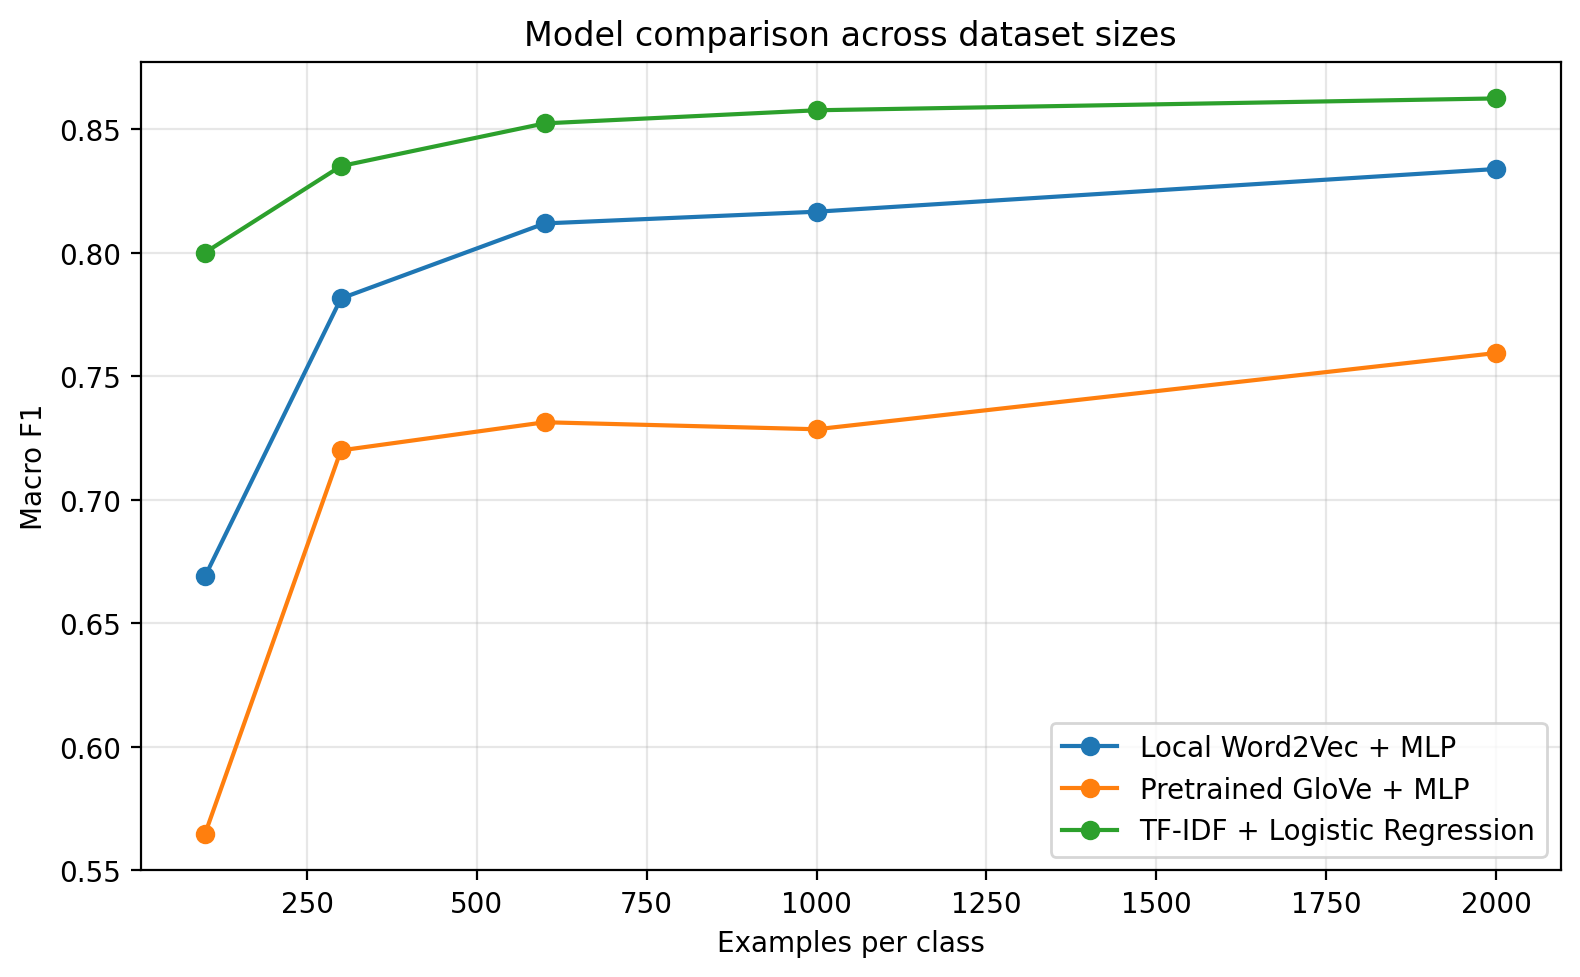
\includegraphics[width=0.88\linewidth]{../artifacts/model_comparison_compact.png}
\caption{Macro F1 across dataset sizes for the three models.}
\label{fig:maincurve}
\end{figure}

The same trend is visible in accuracy. TF--IDF remains the strongest method at every subset size; Local Word2Vec improves substantially with more data; and Pretrained GloVe is consistently the weakest model.

\section{Discussion}
The results support several conclusions.

First, the strongest overall model is the classical baseline. This indicates that consumer complaint classification is heavily driven by surface lexical cues. Product categories can often be inferred from highly informative words and short phrases, and TF--IDF with bigrams captures these patterns effectively. In this setting, sparse lexical features appear more useful than averaged dense semantic vectors.

Second, locally trained embeddings are clearly better than pretrained GloVe. This suggests that domain-specific semantics matter. Financial complaint texts contain recurring terminology and complaint-specific phrasing that may not be represented well by general-domain pretrained vectors. As the amount of in-domain training text increases, Local Word2Vec becomes increasingly competitive, improving from macro F1 of 0.6596 at 100 examples per class to 0.8358 at 2000 examples per class.

Third, the original expectation that pretrained embeddings would help most in the smallest-data regime is not supported by these experiments. Even at 100 examples per class, pretrained GloVe remains behind both TF--IDF and Local Word2Vec. This may be due to two factors: the domain mismatch between general-purpose embeddings and financial complaints, and the simplicity of document representation by plain averaging, which removes important word order and phrase-level information.

Finally, the repeated-run evaluation makes the conclusions more credible. The standard deviations shrink as dataset size grows, especially for TF--IDF, indicating that the ranking of models is stable rather than an artifact of a single random split.

\section{Error Analysis}
To better understand where the strongest model still fails, I performed a qualitative error analysis on the TF--IDF + Logistic Regression run with seed 42. Figure~\ref{fig:cm} shows the confusion matrix for that run. The model performs very well on \textit{Mortgage}, but the largest remaining errors come from classes that share legal and financial vocabulary.

\begin{figure}[H]
\centering
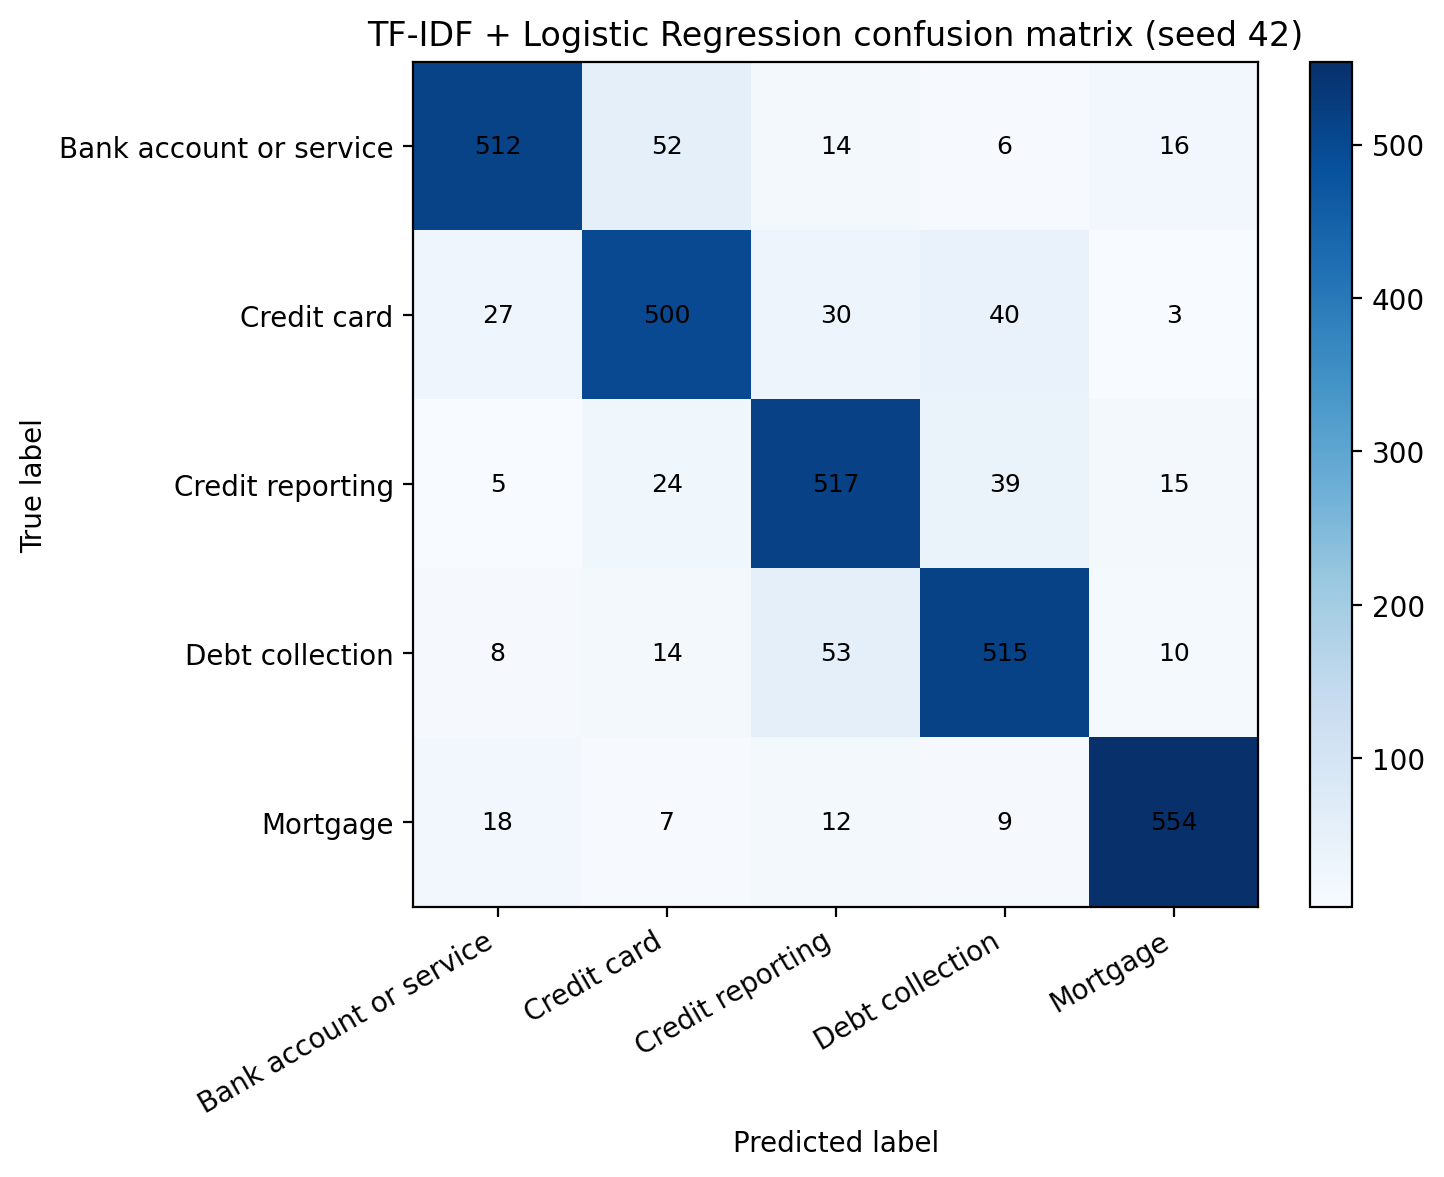
\includegraphics[width=0.82\linewidth]{../artifacts/confusion_matrix_tfidf_seed42.png}
\caption{Confusion matrix for TF--IDF + Logistic Regression on the seed-42 split.}
\label{fig:cm}
\end{figure}

The most frequent confusion pair is \textit{Debt collection} $\rightarrow$ \textit{Credit reporting} (53 cases), followed by \textit{Bank account or service} $\rightarrow$ \textit{Credit card} (52 cases), \textit{Credit card} $\rightarrow$ \textit{Debt collection} (40 cases), and \textit{Credit reporting} $\rightarrow$ \textit{Debt collection} (39 cases). These errors are intuitively plausible because many complaints mention both the underlying account type and downstream effects on credit reports or collections.

\begin{table}[H]
\centering
\caption{Top confusion pairs in the TF--IDF error analysis.}
\label{tab:confusions}
\begin{tabular}{>{\raggedright\arraybackslash}p{0.34\linewidth} >{\raggedright\arraybackslash}p{0.34\linewidth} c}
\toprule
True label & Predicted label & Count \\
\midrule
Debt collection & Credit reporting & 53 \\
Bank account or service & Credit card & 52 \\
Credit card & Debt collection & 40 \\
Credit reporting & Debt collection & 39 \\
Credit card & Credit reporting & 30 \\
\bottomrule
\end{tabular}
\end{table}

A closer look at representative mistakes suggests three main sources of error. First, \textit{Credit reporting} and \textit{Debt collection} complaints often co-occur in the same narrative: a user disputes a debt because it appears on a credit report, or challenges a collection account that is damaging a credit score. Second, \textit{Bank account or service} and \textit{Credit card} narratives overlap whenever the complaint is about payment processing, credit lines, fees, or a bank-branded card. Third, some \textit{Mortgage} complaints mention auto-pay, escrow, or home-equity products in a way that introduces vocabulary also common in general bank-account complaints.

This error analysis reinforces the main conclusion of the project. The TF--IDF baseline is strong because lexical cues are highly informative, but some complaints are genuinely multi-topic. In those borderline cases, the text contains signals for more than one product category, which makes even a strong linear classifier confuse adjacent classes.

\section{Reproducibility}
The project is organized for reproducibility. The repository contains the final notebook used to rebuild the balanced dataset, train all models, run repeated experiments with multiple random seeds, and export summary tables and figures. It also includes a README with run instructions, the report source, the presentation source, and saved artifacts for the main plots and error analysis. Required dependencies are specified in a \texttt{requirements.txt} file. This structure directly supports the course grading criteria for technical correctness, experimental design, insight, and code organization.

\section{Conclusion}
This project compared classical and embedding-based methods for product classification of consumer complaint narratives. The main result is that TF--IDF + Logistic Regression outperforms both embedding-based models across all dataset sizes. Local Word2Vec is consistently stronger than Pretrained GloVe and benefits from additional in-domain data, but neither embedding approach surpasses the classical baseline.

Overall, the experiments show that simpler models remain highly competitive in applied NLP when lexical cues are strong and domain-specific. A natural next step would be to test contextual encoders or stronger sequence models, but within the scope of this mini-project, the current findings already provide a clear and well-supported answer to the research question.

\end{document}
